	  From \eqref{eq:two-pgm},
\begin{align}
\vec{A}-\vec{B} = 
\vec{D}-\vec{C} =  \myvec{-6\\-1}
\end{align}
Hence, $ABCD$ is a parallelogram.
See \figref{fig:chapters/11/10/1/91}.
\begin{figure}[H]
  \centering
   %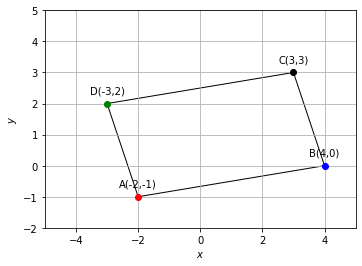
\includegraphics[width=0.75\columnwidth]{chapters/11/10/1/9/figs/paralellogram.png}
   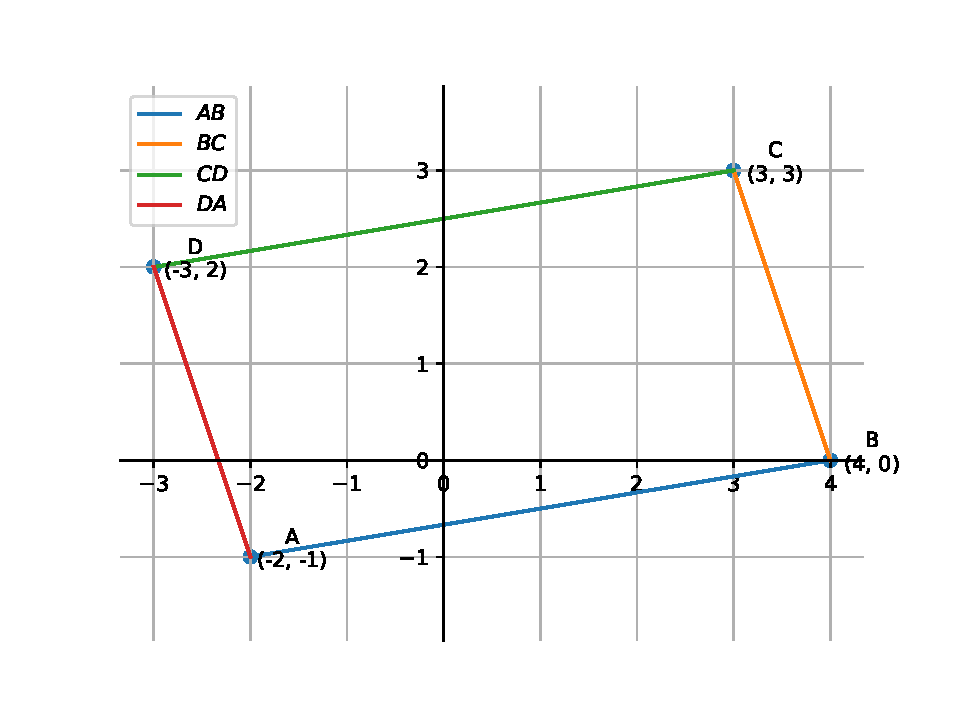
\includegraphics[width=0.75\columnwidth]{chapters/11/10/1/9/figs/fig.pdf}
    \caption{}
     \label{fig:chapters/11/10/1/91}  
\end{figure}



